\clearpage
\section{Umsetzung Benchmark}\label{sec:ThreadUmsetzungBenchmark}
In diesem Kapitel wird die Thread Stack spezifische Benchmark Umsetzung beschrieben. Das gesamte Projekt ist im \href{https://github.com/Rouben94/P6_Software}{Github-Repository\footnote{\url{https://github.com/Rouben94/P6_Software}\cite{github_p6_software_p2p_2020}}} unter dem Ordner \textbf{P6\_Software/Openthread/ Thread\_SDK/custom/P6\_Project/ot\_benchmark/} verfügbar. Ausserdem sind im Ordner \textbf{P6\_Software/Openthread/Thread\_SDK/custom/benchmark\_hex/} die vorkompilierten .zip Dateien abgespeichert, um diese auf den nRF52840 SoC zu flashen. 

\subsection{Openthread Stack Konfiguration}\label{subsec:ThreadStackKonfiguration}
In nachfolgender Tabelle sind alle Parameter aufgelistet, die verwendet werden, um den Openthread Stack mit CoAP Funktion zu konfigurieren.
\begin{table}[h]
	\centering
	\begin{adjustbox}{width=1\textwidth}
		\begin{tabular}{|l|l|l|} 
			\hline
			Stack Init Time                             & 30000 ms                                                                & \begin{tabular}[c]{@{}l@{}}Zeit, die benötigt wird, um den Stack für den Benchmark\\zu initialisieren. Reserve Zeit, um das Routing des \\Netzwerkes durchzuführen. \end{tabular}  \\ 
			\hline
			\multicolumn{1}{l}{}                        & \multicolumn{1}{l}{}                                                    & \multicolumn{1}{l}{}                                                                                                                                                            \\ 
			\hline
			IEEE Channel                                & 15                                                                      & \begin{tabular}[c]{@{}l@{}}Thread Kanal, der verwendet wird, um das Mesh \\aufzubauen.\end{tabular}                                                                               \\ 
			\hline
			Netzwerk Name                               & OpenThread                                                              & Netzwerkname                                                                                                                                                                    \\ 
			\hline
			\textcolor[rgb]{0.275,0.275,0.278}{PAN ID}  & \textcolor[rgb]{0.275,0.275,0.278}{0xABCD}                              & Personal Area Network ID                                                                                                                                                        \\ 
			\hline
			Netzwerkschlüssel                           & \textcolor[rgb]{0.275,0.275,0.278}{0x00112233445566778899AABBCCDDEEFF}  & Wird für das Precomissioning verwendet.                                                                                                                                         \\ 
			\hline
			Radio Modus                                 & radio-on-when-idle                                                      & Das Radio Interface wird nie abgeschaltet.                                                                                                                                      \\ 
			\hline
			Node Type                                   & FTD                                                                     & \begin{tabular}[c]{@{}l@{}}Alle Nodes werden als Full Thread Devices konfiguriert\\und habe entweder eine Parent oder eine Child Rolle.\end{tabular}                            \\ 
			\hline
			Comissioning                                & Auto-Comissioning                                                       & \begin{tabular}[c]{@{}l@{}}Alle Thread Gerät befinden sich nach der Initialisierung \\im gleichen Netzwerk.\end{tabular}                                                        \\ 
			\hline
			\multicolumn{1}{l}{}                        & \multicolumn{1}{l}{}                                                    & \multicolumn{1}{l}{}                                                                                                                                                            \\ 
			\hline
			BSP LED 0                                   & BSP\_LED\_THREAD\_CONNECTION                                            & Zeigt den Verbindungsstatus an.                                                                                                                                                 \\ 
			\hline
			BSP LED 1                                   & BSP\_LED\_THREAD\_COMMISSIONING                                         & Zeigt den Commissioning Status an.                                                                                                                                              \\ 
			\hline
			BSP LED 2                                   & BSP\_LED\_ALERT                                                         & Zeigt an, ob ein Fehler anliegt.                                                                                                                                                \\ 
			\hline
			\multicolumn{1}{l}{}                        & \multicolumn{1}{l}{}                                                    & \multicolumn{1}{l}{}                                                                                                                                                            \\ 
			\hline
			CoAP Port                                   & 0x1633                                                                  & CoAP Port für Nachrichtenübertragung.                                                                                                                                           \\ 
			\hline
			URI Path                                    & bm\_probe                                                               & \begin{tabular}[c]{@{}l@{}}URI konfiguration für die Identifizierung der CoAP \\Benchmark Message\end{tabular}                                                                  \\ 
			\hline
			Group Address                               & ff03::Aktuelle Gruppe                                                   & \begin{tabular}[c]{@{}l@{}}Beim Initialisieren wird sogleich die eingestellte Gruppen~\\Multicast Adresse konfiguriert.\end{tabular}                                            \\
			\hline
		\end{tabular}
	\end{adjustbox}
	\caption{Parameter zu Konfiguration des Stacks}
	\label{tab:ParameterKonfigurationStacks}
\end{table}

\paragraph{Autocomissioning}
Alle Thread Knoten werden mit den Parametern von Tabelle \ref{tab:ParameterKonfigurationStacks} initialisiert. Da die Parameter fest programmiert wurden, verbinden sich alle Knoten direkt in das Netzwerk namens OpenThread. Somit entfällt ein Comissioning-Prozess, was das Aufstarten extrem beschleunigt. Trotzdem ist ein Zeitfenster von 30s hinterlegt, bevor der Benchmark startet, da die einzelnen Knoten zuerst ihre Rolle bestimmen müssen und den Routing-Prozess durchlaufen müssen.

\newpage
\paragraph{Channel Wahl}
Die Openthread API stellt eine automatische Channel Wahl namens Channel Manager zur Verfügung. Der Channel Manager führt ein Qualitätscheck aus und vergleicht die verfügbaren Channels. Nachdem der Channel mit der besten Qualität ausgewählt wurde, wechseln alle Knoten den Channel zu dem vom Channel Manager vorgegebenen Channel. Leider konnte die Funktion nicht ausreichend geprüft werden und der Channelwechsel funktionierte nicht immer bei allen Nodes. Aus diesem Grund wurde der Channel Manager deaktiviert und ein spezifischer Channel ausgewählt, auf dem der Benchmark läuft. Wie in Abbildung \ref{fig:ChannelBandbreite} ersichtlich ist Channel 15 auf der Frequenz 2425MHz am wenigsten von anderen Quellen wie W-Lan oder BLE belastet. Somit wurde Channel 15 als Standard Channel ausgewählt.
\begin{figure}[H]
	\centering
	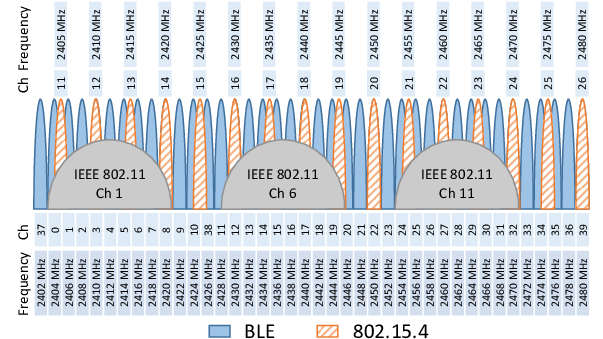
\includegraphics[width=0.7\textwidth]{Channels.png}
	\caption{Channel Bandbreite \cite{zand_fig_nodate}}\label{fig:ChannelBandbreite}
\end{figure}

\subsection{Openthread Stack Initialisierung}\label{subsec:OpenthreadStackInitialisierun}
Der Openthread Stack wird, wie in Abbildung \ref{fig:InitialisierungThreadStack} ersichtlich, mit den bereits erläuterten Parametern von Kapitel \ref{subsec:ThreadStackKonfiguration} initialisiert:

\begin{figure}[H]
	\centering
	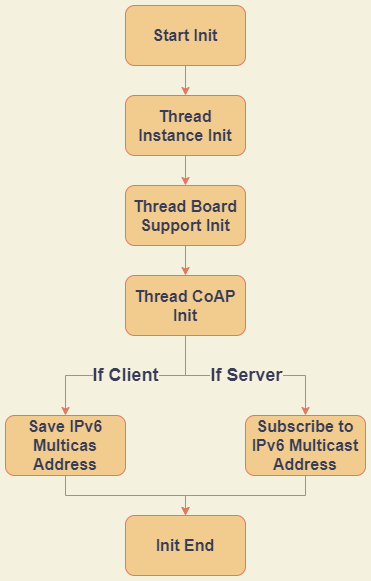
\includegraphics[width=0.3\textwidth]{Initialisierung Thread Stack.png}
	\caption{Initialisierung Thread Stack}\label{fig:InitialisierungThreadStack}
\end{figure}

\newpage
\subsection{CoAP Benchmark Message}\label{subsec:ThreadBenchmarkMessage}
Um die Benchmark Message vom Client an den Server zu senden, wurde ein CoAP-Protokoll implementiert. Das Protokoll ist im Kapitel \ref{subsubsec:CoAP} näher erläutert. Nachfolgend wird beschrieben, welche Funktionen implementiert wurden.

\paragraph{Default Handler} 
Der Default-Handler ist eine Callbackfunktion, die jede CoAP Applikation beinhalten muss. Bei der Initialisierung von CoAP muss eine Callbackfunktion mitgegeben werden. Diese wird aufgerufen, falls die CoAP Nachricht nicht zugeordnet werden kann. Falls letzteres der Fall sein sollte, bedeutet dies zwar, dass die Adresse der Nachricht stimmt, jedoch der Uniform Resource Identifier (URI) der Nachricht nicht registriert wird. Der URI wird verwendet, um die Nachricht zu identifizieren. 

\paragraph{Probe Message Send}
Nur Clientseitig implementiert ist die Funktion \textit{bm\_coap\_probe\_message\_send}. Mit dieser\linebreak Funktion wird eine neue Nachricht generiert und an die entsprechende Multicast Adresse gesendet. Zusätzlich zu der Adresse wird ein CoAP Port benötigt. Dieser ist standartmässig auf die Portadresse \textit{0x1633} festgelegt. Folgende Parameter werden mit der Nachricht gesendet:

\begin{itemize}
	\item \textbf{URI} - bm\_probe
	\item \textbf{Message ID} - Die aktuelle Message ID, um die Nachricht identifizieren zu können. (1 byte)
	\item \textbf{Source Adress} - Die Adresse des Clients, damit in der Auswertung die Gruppenbeziehungen ausgewertet werden können. (2 byte)
	\item \textbf{Payload} - Zusätzliche Payload, die mit zufälligen Daten gefüllt wird (1 - 1021 byte)
\end{itemize}

Bevor die Nachricht gesendet wird, werden folgende Parameter ausgelesen und ins RAM gespeichert:

\begin{table}[H]
	\centering
	\begin{tabular}{|l|l|}
		\hline
		\textbf{Parameter}  & \textbf{Erklärung}                                                                                               \\ \hline
		Source Address      & EID Adresse vom Client                                                                                           \\ \hline
		Destination Address & Zieladresse, an den die Nachricht gesendet wird.                                                                 \\ \hline
		Group Address       & Aktuelle Gruppenadresse, die initialisiert ist.                                                                 \\ \hline
		Message ID          & Aktuelle Message ID                                                                                              \\ \hline
		Network Time        & \begin{tabular}[c]{@{}l@{}}Aktuelle Netzwerk Zeit, die mit der Zeitsynchronisation\\ verfügbar ist.\end{tabular} \\ \hline
		Payload Length      & Zusätzliche Payload, die mitgegeben werden kann.                                                                  \\ \hline
	\end{tabular}
	\caption{Messparameter Client Thread}
	\label{table:MessparameterClientThread}
\end{table}

\newpage
\paragraph{Probe Message Handler}
Um die Benchmark Message auf dem Server zu erhalten, wird eine Callbackfunktion mit dem entsprechenden URI (\textit{bm\_probe}) initialisiert. Wird die Funktion \textit{bm\_probe\_message\_handler} nach Eingang einer validen CoAP Nachricht aufgerufen, so werden folgende Parameter entweder aus der Nachricht ausgelesen oder vom System abgerufen und ins RAM gespeichert:

\begin{table}[H]
	\centering
	\begin{adjustbox}{width=1\textwidth}
		\begin{tabular}{|l|l|l|}
			\hline
			\textbf{Parameter}  & \textbf{Erklärung}                                                                                               & \textbf{In der Payload mitgegeben} \\ \hline
			Source Address      & EID Adresse vom Client                                                                                           & \multicolumn{1}{c|}{X}             \\ \hline
			Destination Address & EID Adresse vom Server                                                                                           &                                    \\ \hline
			Group Address       & Aktuelle Gruppenadresse, die initialisiert ist.                                                                 &                                    \\ \hline
			Message ID          & Aktuelle Message ID                                                                                              & \multicolumn{1}{c|}{X}             \\ \hline
			Network Time        & \begin{tabular}[c]{@{}l@{}}Aktuelle Netzwerk Zeit, die mit der Zeitsynchronisation\\ verfügbar ist.\end{tabular} &                                    \\ \hline
			Payload Length      & Zusätzliche Payload, die mitgegeben werden kann.                                                                  & \multicolumn{1}{c|}{}              \\ \hline
			RSSI                & RSSI Durchschnittswert über alle Hops                                                                            &                                    \\ \hline
			Number od Hops      & Anzahl Hops die die Nachricht genommen hat                                                                       &                                    \\ \hline
		\end{tabular}
	\end{adjustbox}
	\caption{Messparameter Server Thread}
	\label{table:MessparameterServerThread}
\end{table}

\subsection{IPv6 Adressierung}\label{subsec:IPv6Adressierung}
Die einzelnen Knoten im Benchmark Test sollten in Gruppen konfiguriert werden, da dies der Praxis einer Heimautomation entspricht. Dort können verschiedene Schalter mehrere Leuchten ein- und ausschalten. Hierfür bietet sich die Multicast Adressierung von Thread an, da mehrere Nachrichten gleichzeitig versendet werden können, wie im Abschnitt \ref{subsubsec:IPv6Adressierung} beschrieben. Um diese Gruppenadressierung mit Multicast Adressen umzusetzen, wurden 25 verschiedene Adressen vordefiniert:

\begin{table}[H]
	\centering
	\begin{tabular}{|l|l|}
		\hline
		\textbf{Gruppen Nummber} & \textbf{Multicast Adresse} \\ \hline
		1                        & ff03::3                    \\ \hline
		2                        & ff03::4                    \\ \hline
		3                        & ff03::5                    \\ \hline
		4                        & ff03::6                    \\ \hline
		...                      & ...                        \\ \hline
		25                       & ff03::27                   \\ \hline
	\end{tabular}
	\caption{Gruppenadressierung Thread}
	\label{table:GruppenadressierungThread}
\end{table}